% /home/tian/workspace/dpol/polarimeter/docs/code/polarimeter_stastic/polarimeter_stastic.tex
\documentclass[11pt,a4paper]{article}
\usepackage[utf8]{inputenc}
\usepackage[T1]{fontenc}
\usepackage{lmodern}
\usepackage{microtype}
\usepackage[a4paper,margin=2.5cm]{geometry}

\usepackage{amsmath,amssymb,bm}
\usepackage{mathrsfs}
\usepackage{siunitx}
\usepackage{graphicx}
\usepackage{caption}
\usepackage{subcaption}
\usepackage{tikz}
\usepackage{braket}
\usepackage{physics}
\usepackage[hidelinks]{hyperref}

% Put figures in a subdirectory "figures/"
% \graphicspath{{figures/}}

\title{polarimeter}
\author{Tian Baiting}
\date{\today}

\begin{document}
\maketitle
\begin{abstract}
This document presents the principles of the polarimeter and the associated statistical analysis.
\end{abstract}

\section{Theory of Polarimeter Measurements}
\label{sec:theory}

The polarization state of polarized baryon beams, such as deuteron beams, can be monitored by measuring the differential cross-sections of deuteron-proton (d-p) elastic scattering at different angles.

\subsection{Definition of Tensor Polarization}

The deuteron is a spin-$S=1$ system, and its polarization state can be fully described by the spin density operator. The density operator $\hat{\rho}$ characterizes the statistical mixture of pure quantum states:
\begin{equation}
\hat{\rho} = \sum_i Q_i \ket{\phi_i}\bra{\phi_i}
\end{equation}
where $Q_i$ is the probability of the pure state $\ket{\phi_i}$. For a spin-1 deuteron, the density matrix is a $3 \times 3$ Hermitian matrix encompassing both vector and tensor polarization information. Expanding in a Cartesian basis, the vector polarization operators are $\mathscr{P}_i = S_i$, and the tensor polarization operators are $\mathscr{P}_{ij}= 3 S_i S_j - 2I$ (where $I$ is the identity matrix). The density matrix can be expanded as:
\begin{equation}
\begin{aligned}
    \hat{\rho} = \frac{1}{3} \Bigg\{ &I + \frac{3}{2} \left( p_x \mathscr{P}_x + p_y \mathscr{P}_y + p_z \mathscr{P}_z \right) \\  
    &+ \frac{2}{3} \left( p_{xy} \mathscr{P}_{xy} + p_{yz} \mathscr{P}_{yz} + p_{xz} \mathscr{P}_{xz} \right) \\ 
    &+ \frac{1}{3} \left( p_{xx} \mathscr{P}_{xx} + p_{yy} \mathscr{P}_{yy} +p_{zz} \mathscr{P}_{zz} \right) \Bigg\}
\end{aligned}
\end{equation}
where $p_i$ and $p_{ij}$ represent the vector and tensor polarization components of the initial deuteron beam, respectively. Note that since $\mathscr{P}_{x x} + \mathscr{P}_{y y} + \mathscr{P}_{z z} = 0$, these three components are linearly dependent.

\subsection{Polarization Monitoring Method and Cross-Section Formulas}

In quantum mechanics, the initial and final states of a reaction are related by the scattering matrix $M$ ($\ket*{\phi_{\mathrm{f}}} = M \ket*{\phi_{\mathrm{i}}}$), from which the final density matrix is given by:
\begin{equation}
\hat{\rho}_{\mathrm{f}} = M\hat{\rho}_{\mathrm{i}} M^\dagger
\end{equation}
The vector analyzing powers $A_i$ and tensor analyzing powers $A_{ij}$ are defined as follows:
\begin{equation}
    A_i = M \mathscr{P}_i M^\dagger , \quad A_{ij} = \frac{{\rm Tr} (M \mathscr{P}_{ij} M^\dagger)}{{\rm Tr}(MM^\dagger)}
\end{equation}
Considering a polarized beam, the relationship between the polarized differential cross-section and the unpolarized differential cross-section $\sigma_0(\theta) = \frac{1}{3} {\rm Tr}(M M^\dagger)$ can be expressed as:
\begin{equation}
\label{eq:primary_pol_crosssection}
    \sigma = \sigma_0(\theta) \left\{ 1 + \frac{3}{2} \sum_i p_i A_i  + \frac{1}{3} \sum_{ij} p_{ij} A_{ij}\right\} 
\end{equation}

To correspond with experimental measurements, we need to define the coordinate systems and consider parity conservation conditions such as mirror symmetry. As shown in Figure~\ref{fig:frame}, we define the $S$ coordinate system (red) as the projectile helicity frame, and the $S'$ coordinate system (black) as the laboratory beam frame, where the beam is incident along the $z'$ axis.

\begin{figure}[htbp]
\begin{center}
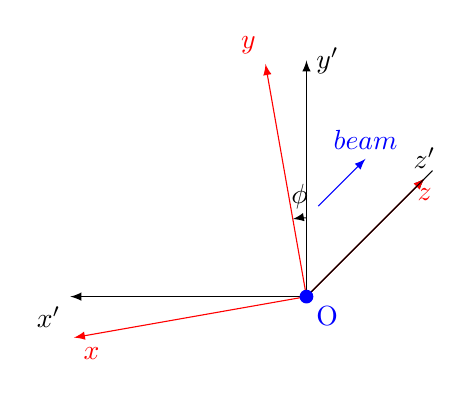
\begin{tikzpicture}[>=latex, x={(1cm,0cm)}, y={(0cm,1cm)}, z={(0.5cm,0.5cm)}]
\draw[->] (0,0,0) -- (-3,0,0) node[below left] {$x'$};
\draw[->] (0,0,0) -- (0,3,0) node[right] {$y'$};
\draw[->] (0,0,0) -- (0,0,3) node[above] {$z'$};
\draw[->,red] (0,0,0) -- (-{3*cos(10)}, -{3*sin(10)}, 0) node[below right] {$x$};
\draw[->,red] (0,0,0) -- ({-3*sin(10)}, {3*cos(10)}, 0) node[above left] {$y$};
\draw[->,red] (0,0,0) -- (0,0,3) node[below] {$z$};
\draw[->,blue] (0,1,0.3) -- (0,1,1.5) node[above]{$beam$};
\draw (0,0,0) -- (0.8,0.8,0) -- (0.8,0.8,1.6) -- cycle;
\draw[->] (0,1,0) arc (90:100:1) node[midway,above] {$\phi$};
\filldraw[blue] (0,0,0) circle (0.08) node[below right] {O};
\end{tikzpicture}
\end{center}
\caption{Schematic diagram of the reference frames. The red axes represent the projectile helicity frame ($S$), with the $xoz$ plane defined as the reaction plane. The black axes represent the laboratory beam frame ($S'$).}
\label{fig:frame}
\end{figure}

After a coordinate transformation and the application of parity conservation conditions, Equation~\ref{eq:primary_pol_crosssection} can be expanded as:
\begin{equation}
\label{eq:polar_crosssection}
\begin{aligned}
    \frac{\sigma(\theta, \phi)}{\sigma_0(\theta)}=1 & +\frac{3}{2}\left(p_{x^{\prime}} \sin \phi+p_{y^{\prime}} \cos \phi\right) A_y(\theta) \\
    &+\frac{2}{3}\left(p_{x^{\prime} z^{\prime}} \cos \phi-p_{y^{\prime} z^{\prime}} \sin \phi\right) A_{x z}(\theta)  \\
    &+\frac{1}{6}\left[\left(p_{x^{\prime} x^{\prime}}-p_{y^{\prime} y^{\prime}}\right) \cos 2 \phi-2 p_{x^{\prime} y^{\prime}} \sin 2 \phi\right] \\
    &\times\left[A_{x x}(\theta)-A_{yy}(\theta)\right] +\frac{1}{2} p_{z^{\prime} z^{\prime}} A_{z z}(\theta) 
\end{aligned}
\end{equation}

\subsection{Polarization Observables and Detector Layout}

Using the above formulas, we can place detectors at the same polar angle $\theta$ but different azimuthal angles $\phi=0^\circ, 90^\circ, 180^\circ, 270^\circ$ (denoted as L, U, R, D for Left, Up, Right, Down, respectively) to monitor the polarization components. The counting rate cross-sections for these four positions are $\sigma_L, \sigma_U, \sigma_R$, and $\sigma_D$, respectively.

For the monitoring of $p_{y'y'}$ (vertical polarization), we define the counting asymmetry observable $R_{LRUD}$:
\begin{equation}
     R_{LRUD} = \frac{N_L+N_R-N_U-N_D}{N_L+N_R+N_U+N_D}= \frac{p_{y'y'}(A_{xx}-A_{yy})}{2p_{y'y'}A_{zz}-4}
\end{equation}
which yields the calculation formula for $p_{y'y'}$:
\begin{equation}
     p_{y'y'} = \frac{R_{LRUD}}{\frac{1}{2} A_{zz} R_{LRUD}-\frac{1}{4}(A_{xx}-A_{yy})}
\label{eq:pyy_observable}
\end{equation}

For the monitoring of the longitudinal polarization $p_{z'z'}$, we establish a relationship using the average differential cross-section $\Bar{\sigma}$ of the four detectors:
\begin{equation}
   \Bar{\sigma}  \equiv \frac{\sigma_L+\sigma_R+\sigma_D+\sigma_U}{4} = \sigma_0 \left(1+\frac{1}{2}p_{z'z'}A_{zz}\right)
\label{eq:pzz_average_detector}
\end{equation}
In practice, to eliminate systemic errors caused by beam intensity fluctuations, the experimental scheme involves simultaneous measurements at two different polar angles ($\theta_1$ and $\theta_2$) to extract their ratio.

\begin{figure}[htbp]
    \centering
    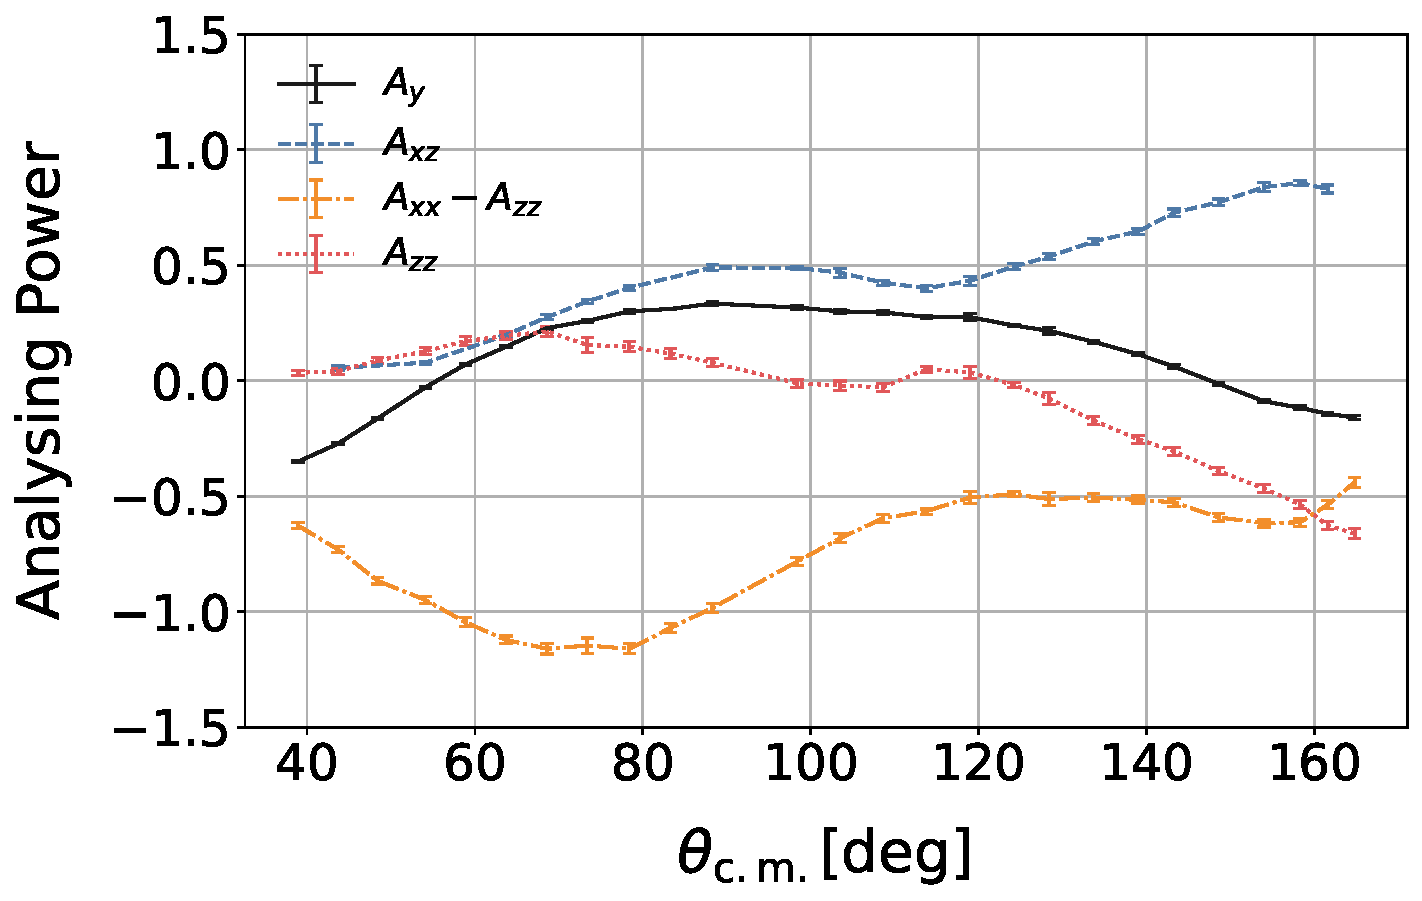
\includegraphics[width=0.45\textwidth]{img/A_zzshow.pdf}
    \caption{Analyzing power as a function of the center-of-mass scattering angle $\theta_{\mathrm{c.m.}}$.}
    \label{fig:analysing_power}
\end{figure}

\begin{figure}[htbp]
    \centering
    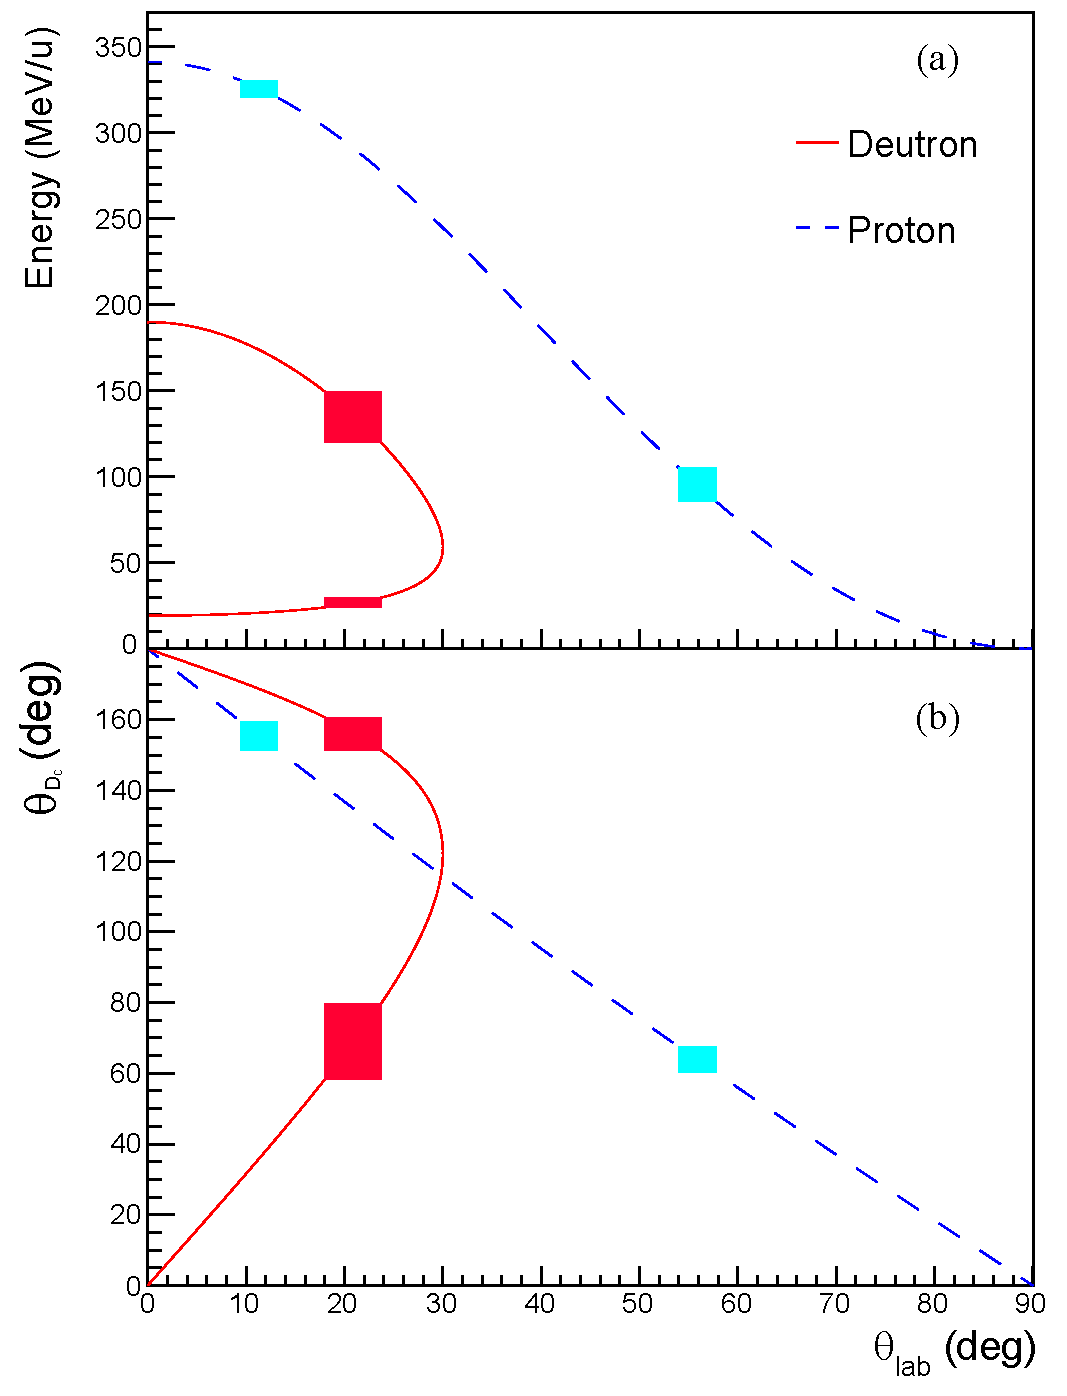
\includegraphics[width=0.45\textwidth]{img/theta_energy.pdf}
    \caption{Correlation of (a) energy and (b) scattering angle for the outgoing deuterons and recoil protons. The colored rectangular regions indicate the designed detector placement angles and coverage ranges.}
    \label{fig:pol_theta_energy}
\end{figure}

Simulation verification shows that the observable ratios and asymmetry indicators have extremely high sensitivity to tensor polarization. Figure~\ref{fig:pzz_counts} and Figure~\ref{fig:pyy_counts} illustrate the effect of $p_{z'z'}$ and $p_{y'y'}$ on their respective observables.

\begin{figure}[htbp]
    \centering
    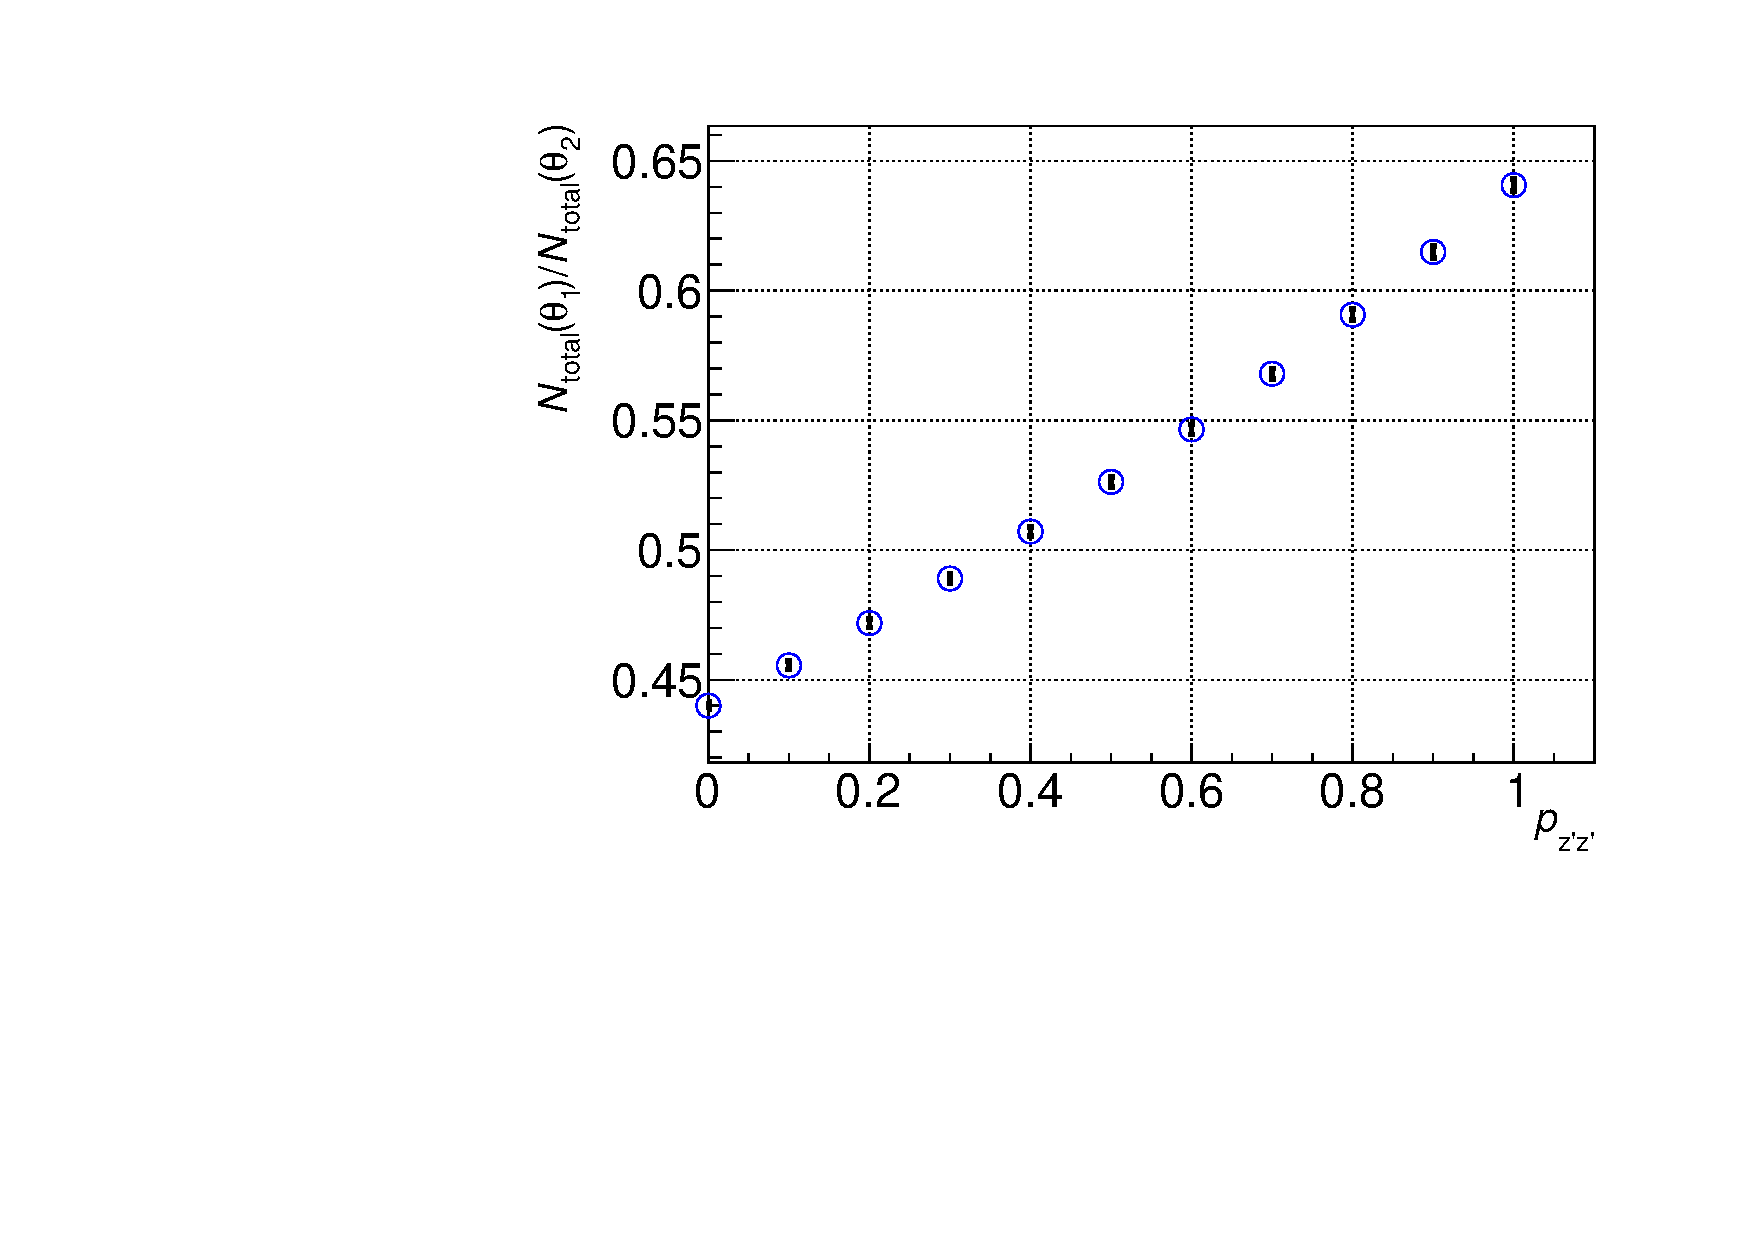
\includegraphics[width=0.45\textwidth]{img/Ratio_vs_pzz.pdf}
    \caption{The relationship between the total count ratio of detectors at $\theta_1$ and $\theta_2$ and the longitudinal tensor polarization $p_{z'z'}$. (The error bars represent the statistical uncertainty under a predetermined 30-minute beam intensity.)}
    \label{fig:pzz_counts}
\end{figure}

\begin{figure}[htbp]
    \centering
    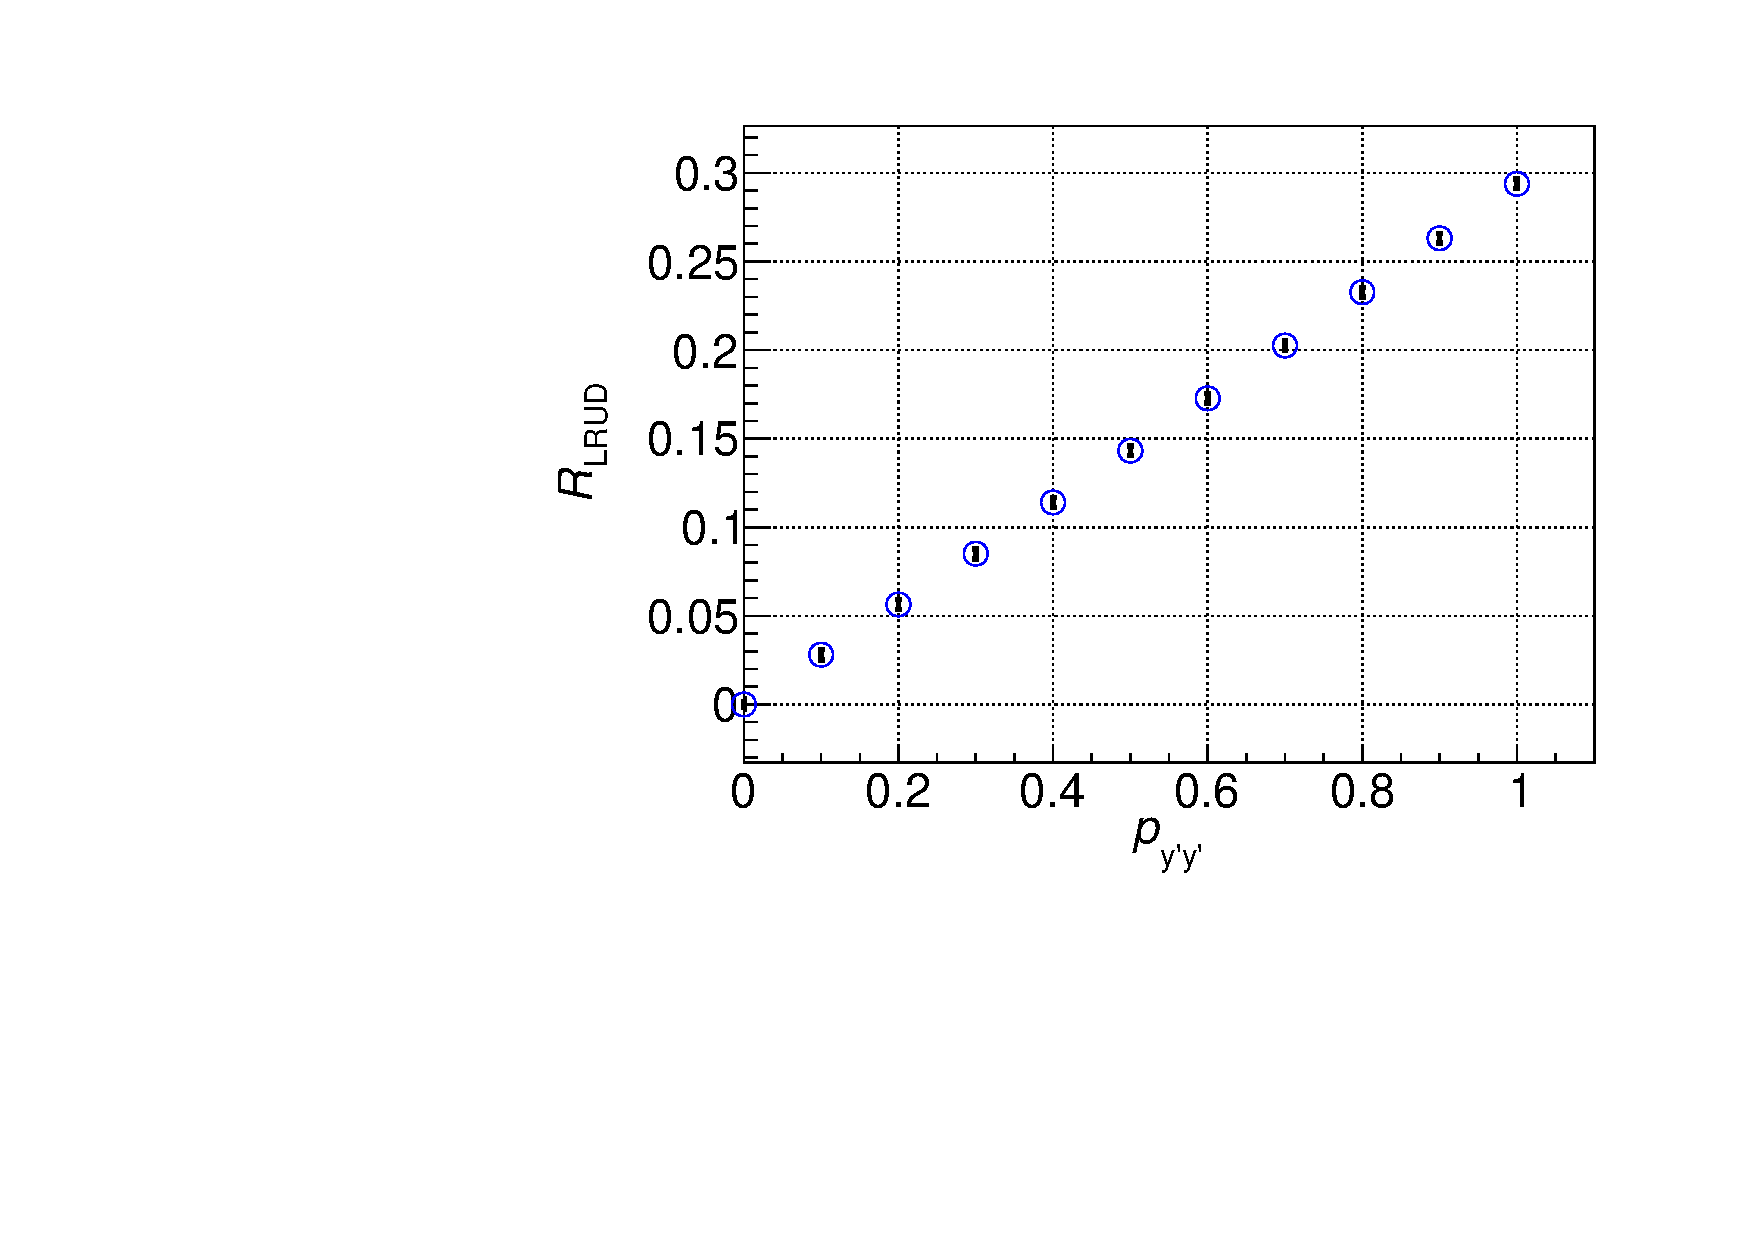
\includegraphics[width=0.45\textwidth]{img/R_LRUD_vs_pyy.pdf}
    \caption{The relationship between the asymmetry observable $R_{LRUD}$ and the vertical polarization component $p_{y'y'}$ (error bars correspond to the predetermined statistical uncertainty).}
    \label{fig:pyy_counts}
\end{figure}


\section{default config}
This section records the numerical setup used by the current \texttt{default.ini} scenario. The batch workflow scans three beam times (\SI{10}{min}, \SI{1}{h}, and \SI{3}{h}); the discussion and figures below use the \SI{3}{h} products as the representative case, while the copied generated artifacts are stored under \texttt{./generated/default/...} with the same analysis-directory structure as \texttt{code/output/default/...}.

\begin{table}[htbp]
    \centering
    \caption{Beam, target, run, and scan configuration from \texttt{code/config/default.ini}.}
    \label{tab:default_config_main}
    \begin{tabular}{lll}
        \hline
        Block & Parameter & Value \\
        \hline
        Beam & Deuteron kinetic energy & \SI{380.0}{MeV} \\
        Beam & Beam current & \SI{1.6e-12}{A}= \SI{1e7}{pps} \\
        Beam & Beam-particle count at \SI{3}{h} & $N_{\mathrm{beam}} = It/e = 1.079\times 10^{11}$ \\
        Target & Areal density & \SI{10000}{g.m^{-2}} \\
        Target & Effective molar mass & \SI{14.0}{g.mol^{-1}} \\
        Run & Duration list & \SIlist{600;3600;10800}{s} \\
        Scan & Polarization grid & 11 points with step 0.1 \\
        Coverage & $(\theta,\phi)$ bins & $360\times 360$ \\
        \hline
    \end{tabular}
\end{table}

\begin{table}[htbp]
    \centering
    \caption{Custom detector layout used by the scans discussed in this section.}
    \label{tab:default_config_layout}
    \begin{tabular}{lll}
        \hline
        Arm & Quantity & Value \\
        \hline
        Proton arm 1 & $\theta_{\mathrm{lab}}$ & \SI{53.4}{\degree} \\
        Proton arm 2 & $\theta_{\mathrm{lab}}$ & \SI{11.2}{\degree} \\
        Proton arms & Distance & \SI{620}{mm} \\
        Proton arms & Active size $(\theta,\phi)$ & \SI{40}{mm} $\times$ \SI{40}{mm} \\
        Deuteron arm & $\theta_{\mathrm{lab}}$ & \SI{20.9}{\degree} \\
        Deuteron arm & Distance & \SI{400}{mm} \\
        Deuteron arm & Active size $(\theta,\phi)$ & \SI{40}{mm} $\times$ \SI{40}{mm} \\
        \hline
    \end{tabular}
\end{table}

For the forward model used by the code, every observable is built from expected counts
\begin{equation}
\label{eq:count_forward_model}
    \lambda(\alpha) =
    M\,N_{\mathrm{target}}\,N_{\mathrm{beam}}
    \int_{\Omega}
    \frac{d\sigma}{d\Omega}(\theta,\phi)\,
    W(\theta,\phi;\alpha)\,d\Omega,
\end{equation}
where $\alpha$ denotes either $p_{zz}$ or $p_{y'y'}$, $M$ is the sector multiplier applied after integrating one explicit detector opening, and $\Omega$ is the accepted solid-angle region in the c.m.\ frame. In the plots, two uncertainty styles are shown: ``stat only'' and ``stat plus $T$'', where the second one includes the propagated tensor-analyzing-power uncertainty in quadrature.

\section{statistic}

\subsection{polariztion rate to count}
\label{sec:forward_counts}

\subsubsection{\texorpdfstring{$p_{zz}$ from paired $N_1/N_2$ observables}{pzz from paired N1/N2 observables}}

For the longitudinal tensor polarization scans, the implementation evaluates two expected counts,
\begin{equation}
\label{eq:pzz_pair_counts}
    \lambda_1(p_{zz}) = a_1 + b_1 p_{zz},
    \qquad
    \lambda_2(p_{zz}) = a_2 + b_2 p_{zz},
\end{equation}
and uses their ratio
\begin{equation}
\label{eq:pzz_pair_ratio}
    R_{12}(p_{zz}) = \frac{N_1}{N_2}.
\end{equation}
The three implemented $p_{zz}$ observables are:
\begin{enumerate}
    \item Proton single-arm ratio:
    \begin{equation}
        N_1 = 4\times N_p(\theta_{\mathrm{lab}}=\SI{53.4}{\degree}),
        \qquad
        N_2 = 4\times N_p(\theta_{\mathrm{lab}}=\SI{11.2}{\degree}).
    \end{equation}
    \item Deuteron single-arm forward/backward ratio:
    \begin{equation}
        N_1 = 4\times N_d(\theta_{\mathrm{lab}}=\SI{20.9}{\degree},\mathrm{forward}),
        \qquad
        N_2 = 4\times N_d(\theta_{\mathrm{lab}}=\SI{20.9}{\degree},\mathrm{backward}).
    \end{equation}
    \item Coupled proton--deuteron coincidence ratio:
    \begin{equation}
        N_1 = N_{p+d}\!\left(\Omega_p^{(1)} \cap \Omega_d^{\mathrm{forward}}\right),
        \qquad
        N_2 = N_{p+d}\!\left(\Omega_p^{(2)} \cap \Omega_d^{\mathrm{backward}}\right).
    \end{equation}
\end{enumerate}
The coincidence mode is the missing coupled observable requested in the implementation update: both $N_1$ and $N_2$ are evaluated only on the c.m.\ overlap accepted simultaneously by the proton and deuteron branches.

\begin{figure}[htbp]
    \centering
    \begin{subfigure}[t]{0.32\textwidth}
        \centering
        
\includegraphics[width=\linewidth]{./generated/default/ratio_proton/3h/N_total4_vs_pzz_stat_plus_T.pdf}
        \caption{Proton single-arm counts.}
    \end{subfigure}
    \begin{subfigure}[t]{0.32\textwidth}
        \centering
        
\includegraphics[width=\linewidth]{./generated/default/ratio_deuteron/3h/N_total4_vs_pzz_stat_plus_T.pdf}
        \caption{Deuteron forward/backward counts.}
    \end{subfigure}
    \begin{subfigure}[t]{0.32\textwidth}
        \centering
        
\includegraphics[width=\linewidth]{./generated/default/ratio_coincidence/3h/N_total4_vs_pzz_stat_plus_T.pdf}
        \caption{Coupled $p+d$ coincidence counts.}
    \end{subfigure}
    \caption{Count-level forward response for the three $p_{zz}$ observables at \SI{3}{h}, including both statistical and tensor-analyzing-power uncertainties.}
    \label{fig:pzz_count_triplet}
\end{figure}

\begin{figure}[htbp]
    \centering
    \begin{subfigure}[t]{0.32\textwidth}
        \centering
        
\includegraphics[width=\linewidth]{./generated/default/ratio_proton/3h/Ratio_vs_pzz_stat_plus_T.pdf}
        \caption{Proton single-arm ratio.}
    \end{subfigure}
    \begin{subfigure}[t]{0.32\textwidth}
        \centering
        
\includegraphics[width=\linewidth]{./generated/default/ratio_deuteron/3h/Ratio_vs_pzz_stat_plus_T.pdf}
        \caption{Deuteron forward/backward ratio.}
    \end{subfigure}
    \begin{subfigure}[t]{0.32\textwidth}
        \centering
        
\includegraphics[width=\linewidth]{./generated/default/ratio_coincidence/3h/Ratio_vs_pzz_stat_plus_T.pdf}
        \caption{Coupled $p+d$ coincidence ratio.}
    \end{subfigure}
    \caption{The corresponding $N_1/N_2$ observables versus $p_{zz}$ at \SI{3}{h}. For the copied outputs, the ratio changes from 0.3594 to 0.5266 for the proton mode, from 3.7653 to 5.4907 for the deuteron mode, and from 0.4259 to 0.6240 for the coupled coincidence mode.}
    \label{fig:pzz_ratio_triplet}
\end{figure}

\subsubsection{\texorpdfstring{$p_{y'y'}$ from $N_{LR}$ and $N_{UD}$}{pyy from NLR and NUD}}

For the vertical tensor polarization scans, the code builds left-right and up-down expectations
\begin{equation}
\label{eq:pyy_lrud_counts}
\begin{aligned}
    \lambda_{LR}(p_{y'y'}) &\propto \int_{\Omega_{LR}}
    \frac{d\sigma}{d\Omega}\left(
        1 - \frac{\sqrt{3}}{2}T_{22}p_{y'y'} - \frac{\sqrt{2}}{4}T_{20}p_{y'y'}
    \right)d\Omega, \\
    \lambda_{UD}(p_{y'y'}) &\propto \int_{\Omega_{UD}}
    \frac{d\sigma}{d\Omega}\left(
        1 + \frac{\sqrt{3}}{2}T_{22}p_{y'y'} - \frac{\sqrt{2}}{4}T_{20}p_{y'y'}
    \right)d\Omega,
\end{aligned}
\end{equation}
and forms the asymmetry
\begin{equation}
\label{eq:pyy_lrud_ratio_impl}
    R_{LRUD} = \frac{N_{LR} - N_{UD}}{N_{LR} + N_{UD}}.
\end{equation}
Two variants are now documented:
\begin{enumerate}
    \item Proton-only LR/UD:
    \begin{equation}
        N_{LR} = 2\times N_p(\mathrm{LR\ sector}, \theta_{\mathrm{lab}}=\SI{53.4}{\degree}),
        \qquad
        N_{UD} = 2\times N_p(\mathrm{UD\ sector}, \theta_{\mathrm{lab}}=\SI{53.4}{\degree}).
    \end{equation}
    \item Coupled proton--deuteron gated LR/UD:
    \begin{equation}
        N_{LR} = 2\times N_{p+d}(\Omega_{LR}^{p,1}\cap \Omega_d^{\mathrm{forward}}),
        \qquad
        N_{UD} = 2\times N_{p+d}(\Omega_{UD}^{p,1}\cap \Omega_d^{\mathrm{forward}}).
    \end{equation}
\end{enumerate}
For the present default geometry, the copied \texttt{summary.csv} and \texttt{scan\_points.csv} show that the proton-only and coincidence-gated LR/UD curves are numerically identical. This is not a general analytical identity; it indicates that, for this specific layout, the deuteron-forward coincidence gate does not further reduce the proton-arm-1 c.m.\ acceptance.

\begin{figure}[htbp]
    \centering
    \begin{subfigure}[t]{0.48\textwidth}
        \centering
        
\includegraphics[width=\linewidth]{./generated/default/lrud_scan/3h/N_LR_N_UD_vs_pyy_stat_plus_T.pdf}
        \caption{Proton-only LR/UD counts.}
    \end{subfigure}
    \begin{subfigure}[t]{0.48\textwidth}
        \centering
        
\includegraphics[width=\linewidth]{./generated/default/lrud_coincidence/3h/N_LR_N_UD_vs_pyy_stat_plus_T.pdf}
        \caption{Coupled $p+d$ gated LR/UD counts.}
    \end{subfigure}
    \caption{Count-level forward response for the two $p_{y'y'}$ observables at \SI{3}{h}.}
    \label{fig:pyy_count_pair}
\end{figure}

\begin{figure}[htbp]
    \centering
    \begin{subfigure}[t]{0.48\textwidth}
        \centering
        
\includegraphics[width=\linewidth]{./generated/default/lrud_scan/3h/R_LRUD_vs_pyy_stat_plus_T.pdf}
        \caption{Proton-only asymmetry.}
    \end{subfigure}
    \begin{subfigure}[t]{0.48\textwidth}
        \centering
        
\includegraphics[width=\linewidth]{./generated/default/lrud_coincidence/3h/R_LRUD_vs_pyy_stat_plus_T.pdf}
        \caption{Coupled $p+d$ gated asymmetry.}
    \end{subfigure}
    \caption{The LR/UD asymmetry used to infer $p_{y'y'}$. In the present default geometry the two curves overlap, with $R_{LRUD}$ rising from 0 to 0.3039 across the scan.}
    \label{fig:pyy_ratio_pair}
\end{figure}

\subsubsection{Duration dependence: \SI{10}{min}, \SI{1}{h}, and \SI{3}{h}}

The central values of the forward observables do not depend on beam time, but the uncertainty bars tighten as the accumulated beam dose grows. The \SI{3}{h} figures above are retained as the cleanest representative plots. To make the short-run and medium-run cases explicit in this subsection as well, the full set of observable-level time-scan figures is collected below for all implemented $p_{zz}$ and $p_{y'y'}$ modes.

\begin{figure}[htbp]
    \centering
    \begin{subfigure}[t]{0.32\textwidth}
        \centering
        
\includegraphics[width=\linewidth]{./generated/default/ratio_proton/10min/Ratio_vs_pzz_stat_plus_T.pdf}
        \caption{\SI{10}{min}.}
    \end{subfigure}
    \begin{subfigure}[t]{0.32\textwidth}
        \centering
        
\includegraphics[width=\linewidth]{./generated/default/ratio_proton/1h/Ratio_vs_pzz_stat_plus_T.pdf}
        \caption{\SI{1}{h}.}
    \end{subfigure}
    \begin{subfigure}[t]{0.32\textwidth}
        \centering
        
\includegraphics[width=\linewidth]{./generated/default/ratio_proton/3h/Ratio_vs_pzz_stat_plus_T.pdf}
        \caption{\SI{3}{h}.}
    \end{subfigure}
    \caption{Beam-time dependence of the proton single-arm $N_1/N_2$ observable for $p_{zz}$.}
    \label{fig:pzz_duration_ratio_proton}
\end{figure}

\begin{figure}[htbp]
    \centering
    \begin{subfigure}[t]{0.32\textwidth}
        \centering
        
\includegraphics[width=\linewidth]{./generated/default/ratio_deuteron/10min/Ratio_vs_pzz_stat_plus_T.pdf}
        \caption{\SI{10}{min}.}
    \end{subfigure}
    \begin{subfigure}[t]{0.32\textwidth}
        \centering
        
\includegraphics[width=\linewidth]{./generated/default/ratio_deuteron/1h/Ratio_vs_pzz_stat_plus_T.pdf}
        \caption{\SI{1}{h}.}
    \end{subfigure}
    \begin{subfigure}[t]{0.32\textwidth}
        \centering
        
\includegraphics[width=\linewidth]{./generated/default/ratio_deuteron/3h/Ratio_vs_pzz_stat_plus_T.pdf}
        \caption{\SI{3}{h}.}
    \end{subfigure}
    \caption{Beam-time dependence of the deuteron forward/backward $N_1/N_2$ observable for $p_{zz}$.}
    \label{fig:pzz_duration_ratio_deuteron}
\end{figure}

\begin{figure}[htbp]
    \centering
    \begin{subfigure}[t]{0.32\textwidth}
        \centering
        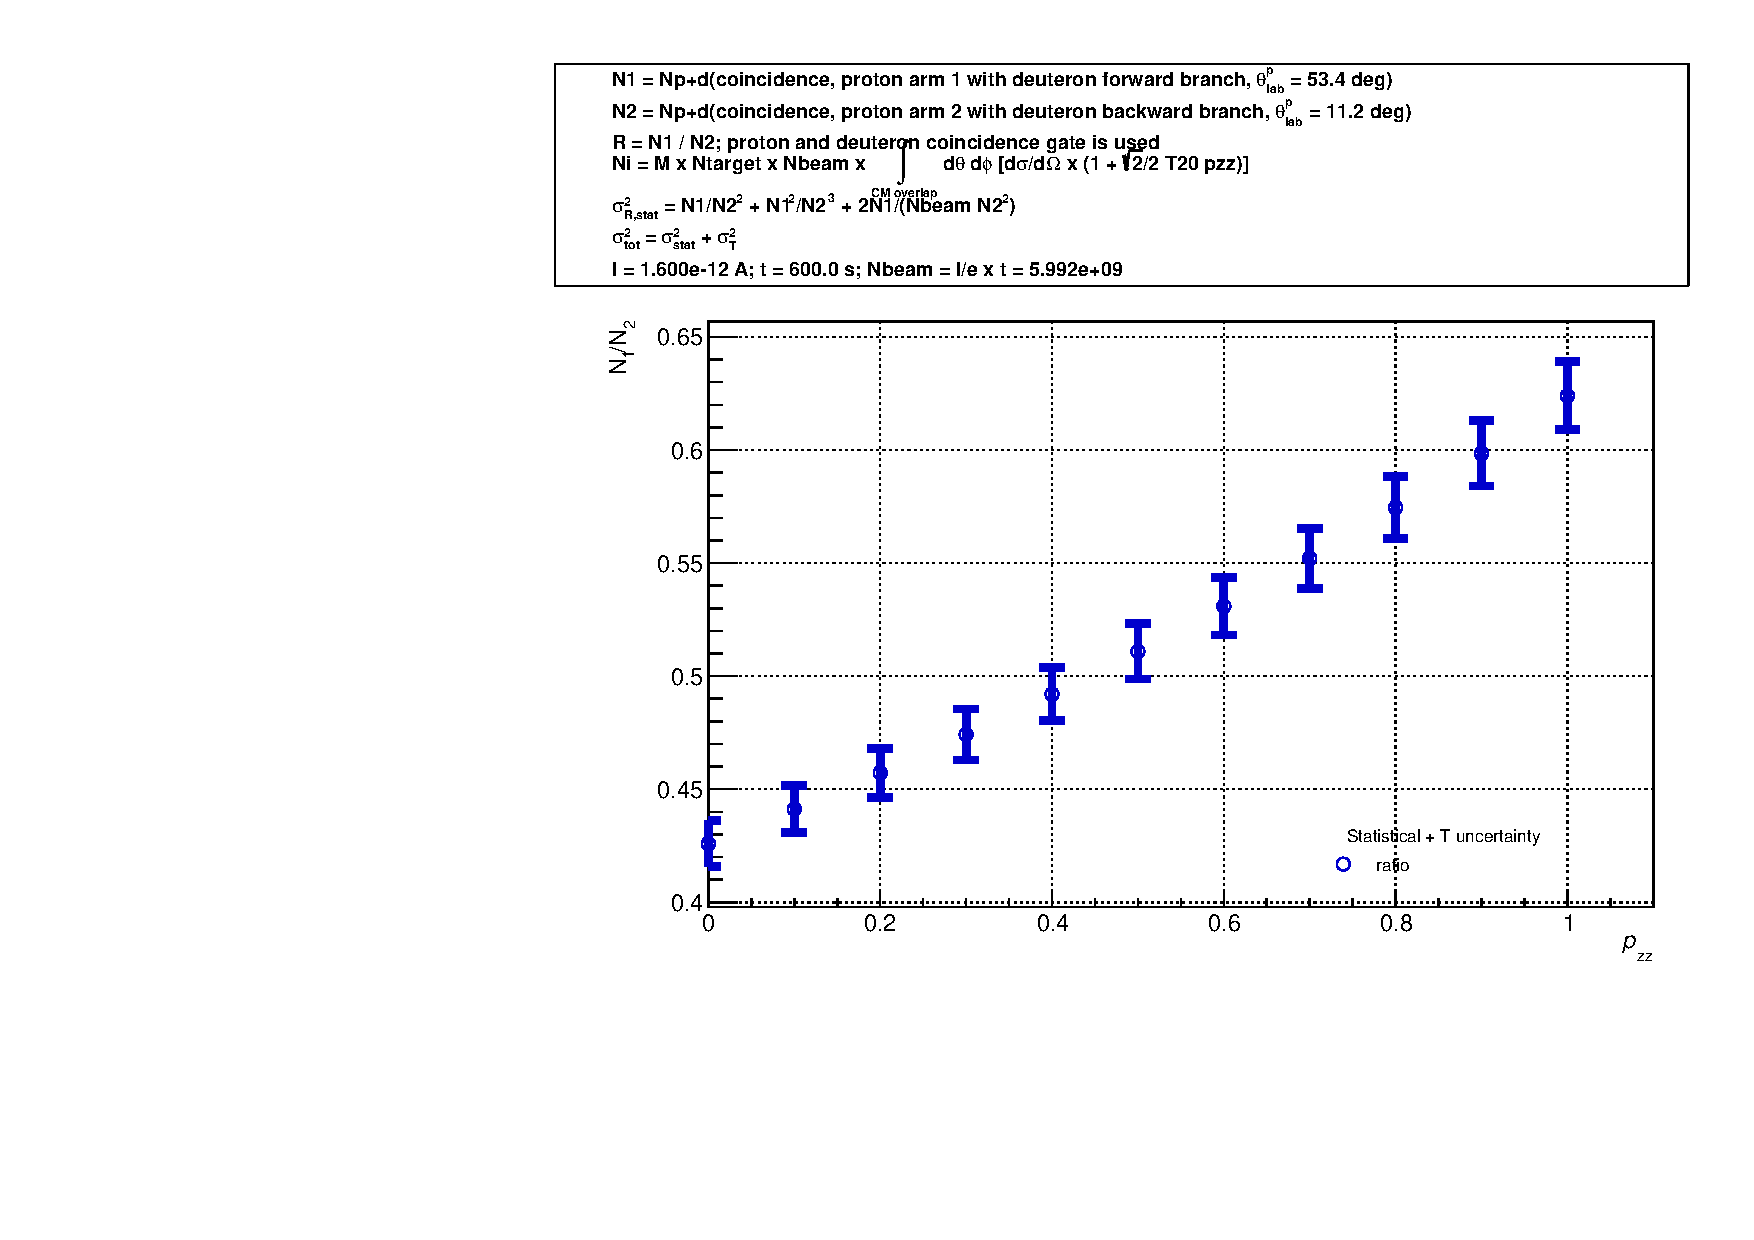
\includegraphics[width=\linewidth]{./generated/default/ratio_coincidence/10min/Ratio_vs_pzz_stat_plus_T.pdf}
        \caption{\SI{10}{min}.}
    \end{subfigure}
    \begin{subfigure}[t]{0.32\textwidth}
        \centering
        
\includegraphics[width=\linewidth]{./generated/default/ratio_coincidence/1h/Ratio_vs_pzz_stat_plus_T.pdf}
        \caption{\SI{1}{h}.}
    \end{subfigure}
    \begin{subfigure}[t]{0.32\textwidth}
        \centering
        
\includegraphics[width=\linewidth]{./generated/default/ratio_coincidence/3h/Ratio_vs_pzz_stat_plus_T.pdf}
        \caption{\SI{3}{h}.}
    \end{subfigure}
    \caption{Beam-time dependence of the coupled $p+d$ coincidence $N_1/N_2$ observable for $p_{zz}$. The central curve is unchanged, while the error bars shrink with increasing dose.}
    \label{fig:pzz_duration_ratio}
\end{figure}

\begin{figure}[htbp]
    \centering
    \begin{subfigure}[t]{0.32\textwidth}
        \centering
        
\includegraphics[width=\linewidth]{./generated/default/lrud_scan/10min/R_LRUD_vs_pyy_stat_plus_T.pdf}
        \caption{\SI{10}{min}.}
    \end{subfigure}
    \begin{subfigure}[t]{0.32\textwidth}
        \centering
        
\includegraphics[width=\linewidth]{./generated/default/lrud_scan/1h/R_LRUD_vs_pyy_stat_plus_T.pdf}
        \caption{\SI{1}{h}.}
    \end{subfigure}
    \begin{subfigure}[t]{0.32\textwidth}
        \centering
        
\includegraphics[width=\linewidth]{./generated/default/lrud_scan/3h/R_LRUD_vs_pyy_stat_plus_T.pdf}
        \caption{\SI{3}{h}.}
    \end{subfigure}
    \caption{Beam-time dependence of the proton-only LR/UD asymmetry for $p_{y'y'}$.}
    \label{fig:pyy_duration_ratio_proton}
\end{figure}

\begin{figure}[htbp]
    \centering
    \begin{subfigure}[t]{0.32\textwidth}
        \centering
        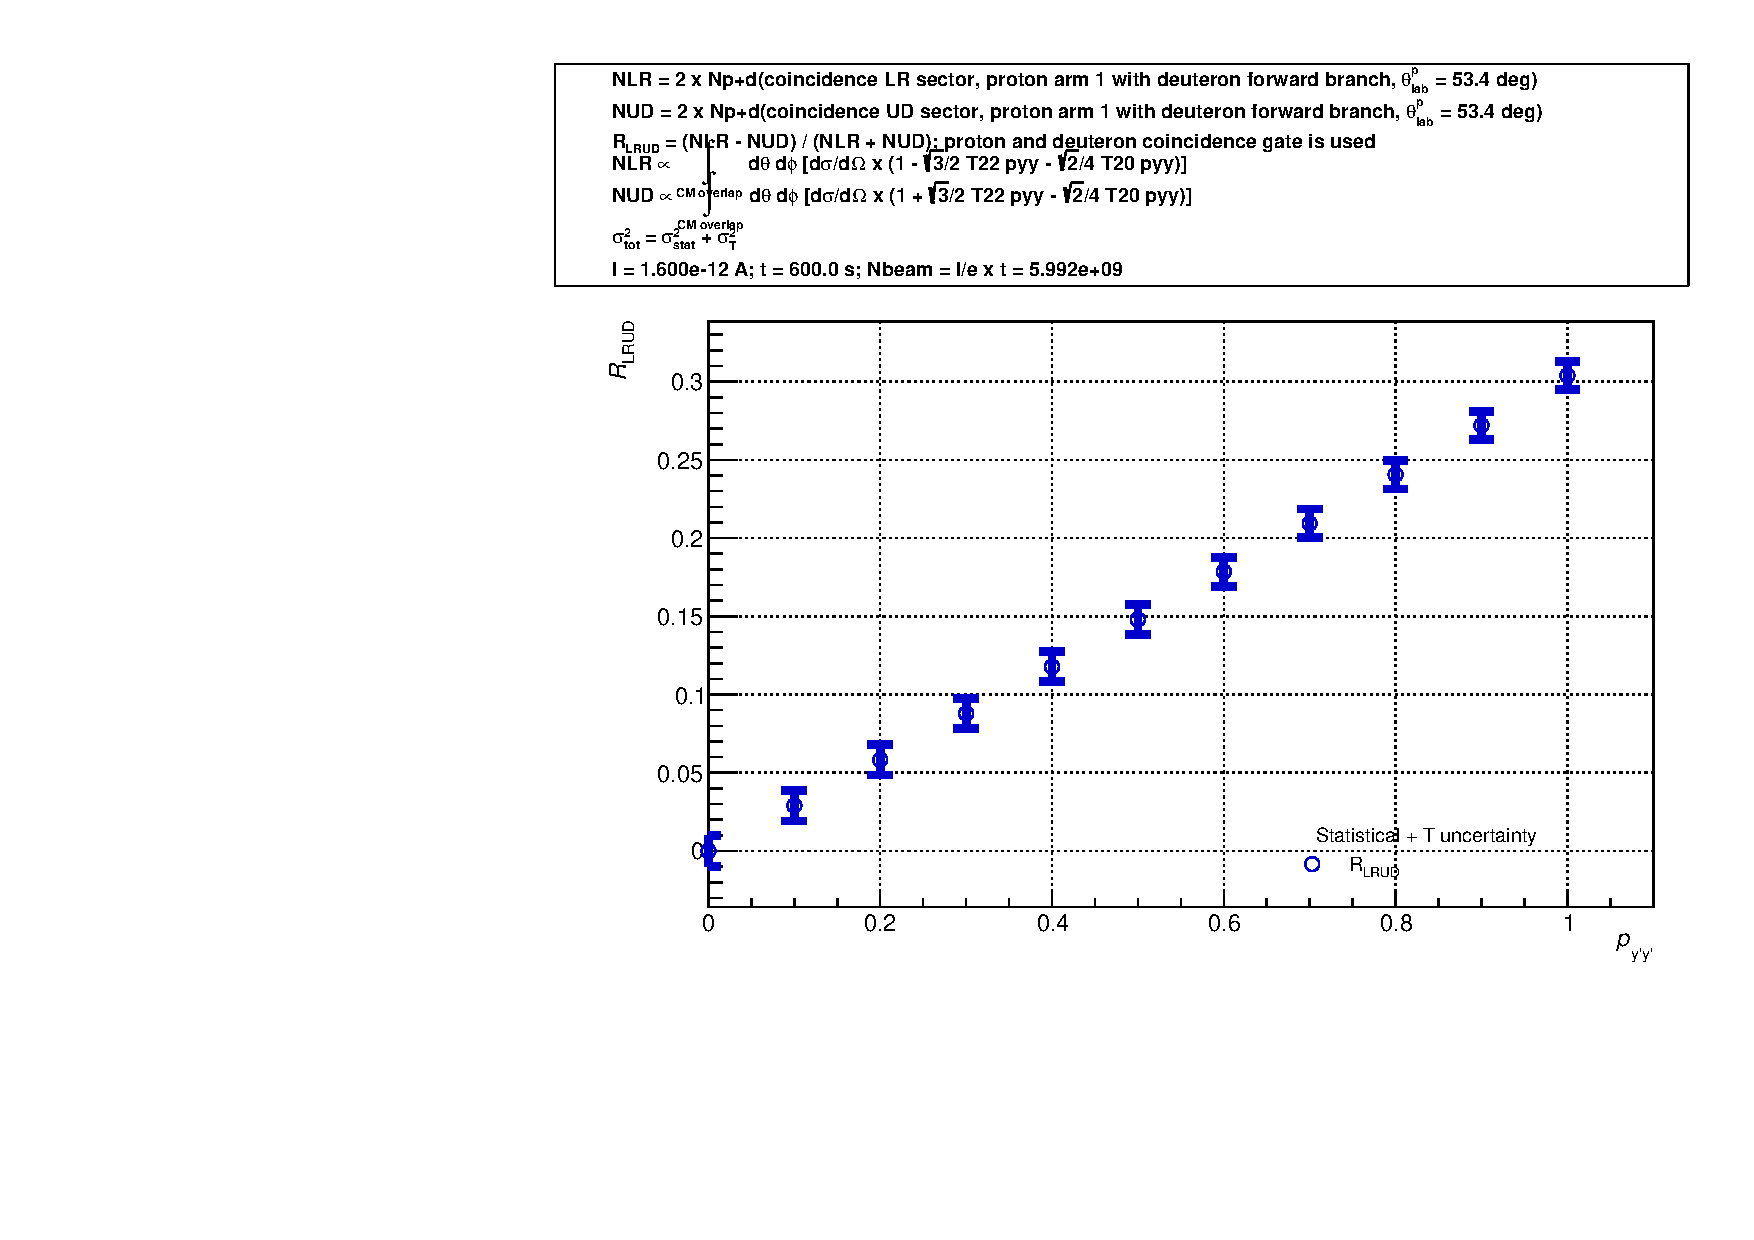
\includegraphics[width=\linewidth]{./generated/default/lrud_coincidence/10min/R_LRUD_vs_pyy_stat_plus_T.pdf}
        \caption{\SI{10}{min}.}
    \end{subfigure}
    \begin{subfigure}[t]{0.32\textwidth}
        \centering
        
\includegraphics[width=\linewidth]{./generated/default/lrud_coincidence/1h/R_LRUD_vs_pyy_stat_plus_T.pdf}
        \caption{\SI{1}{h}.}
    \end{subfigure}
    \begin{subfigure}[t]{0.32\textwidth}
        \centering
        
\includegraphics[width=\linewidth]{./generated/default/lrud_coincidence/3h/R_LRUD_vs_pyy_stat_plus_T.pdf}
        \caption{\SI{3}{h}.}
    \end{subfigure}
    \caption{Beam-time dependence of the coupled $p+d$ gated LR/UD asymmetry for $p_{y'y'}$.}
    \label{fig:pyy_duration_ratio}
\end{figure}

\subsection{from count to polarization rate}
\label{sec:mle_inverse}

The inverse problem in the code is solved by maximum likelihood estimation (MLE). For every paired observable, the forward model supplies two expected counts $\lambda_1(\alpha)$ and $\lambda_2(\alpha)$, with $\alpha = p_{zz}$ or $p_{y'y'}$. Conditioning on the observed total count $N = k_1 + k_2$ removes the normalization nuisance and yields the conditional binomial likelihood
\begin{equation}
\label{eq:pair_binomial_likelihood}
    \pi(\alpha) = \frac{\lambda_1(\alpha)}{\lambda_1(\alpha) + \lambda_2(\alpha)},
    \qquad
    \ln \mathcal{L}(\alpha)
    = k_1 \ln \pi(\alpha) + k_2 \ln \left[1 - \pi(\alpha)\right].
\end{equation}
The MLE is
\begin{equation}
\label{eq:mle_definition}
    \hat{\alpha} = \arg\max_{\alpha \in [0,1]} \ln \mathcal{L}(\alpha),
\end{equation}
and the confidence intervals are extracted from the profile-likelihood drop
\begin{equation}
\label{eq:profile_interval}
    -2\left[\ln \mathcal{L}(\alpha) - \ln \mathcal{L}(\hat{\alpha})\right]
    \le \Delta \chi^2,
    \qquad
    \Delta \chi^2 =
    \begin{cases}
        1.0, & 68\% \\
        3.84, & 95\%.
    \end{cases}
\end{equation}
This is exactly the estimator used for all paired $N_1/N_2$ and $R_{LRUD}$ inversions. The separate coincidence-total diagnostic uses a Poisson likelihood, $\ln\mathcal{L} = N\ln\lambda(\alpha)-\lambda(\alpha)-\ln N!$, but the main coupled observables requested here all use Equation~\ref{eq:pair_binomial_likelihood}.

For the ``Inferred\_*\_vs\_true\_*'' scans, the horizontal-axis true polarization (``true\_p'') is the forward-model input used to compute deterministic expected counts and deterministic expected observables:
$k_1 \equiv \lambda_1(\alpha_{\mathrm{true}})$, $k_2 \equiv \lambda_2(\alpha_{\mathrm{true}})$, and correspondingly $R_{\mathrm{exp}}(\alpha_{\mathrm{true}})$ (ratio or asymmetry). No additional Poisson/binomial random sampling is applied in this step. The inference stage then treats these expected observables as pseudo-observations and inverts them with the same likelihood model to recover $\hat{\alpha}$ and profile-likelihood intervals.

\begin{table}[htbp]
    \centering
    \caption{Representative \SI{3}{h} inverse-inference performance from the copied \texttt{inference\_scan.csv} files. The interval widths are evaluated at the upper scan endpoint.}
    \label{tab:inference_summary}
    \small
    \begin{tabular}{llll}
        \hline
        Observable & Forward observable at $p=1$ & 68\% CI width & 95\% CI width \\
        \hline
        $p_{zz}$ proton single-arm & $N_1/N_2 = 0.5266$ & 0.00655 & 0.01284 \\
        $p_{zz}$ deuteron single-arm & $N_1/N_2 = 5.4907$ & 0.00423 & 0.00828 \\
        $p_{zz}$ coupled $p+d$ coincidence & $N_1/N_2 = 0.6240$ & 0.01352 & 0.02654 \\
        $p_{y'y'}$ proton-only LR/UD & $R_{LRUD} = 0.3039$ & 0.00717 & 0.01407 \\
        $p_{y'y'}$ coupled $p+d$ LR/UD & $R_{LRUD} = 0.3039$ & 0.00717 & 0.01407 \\
        \hline
    \end{tabular}
\end{table}

\begin{table}[htbp]
    \centering
    \caption{Beam-time dependence of the coupled-observable precision. The forward observable is evaluated at the upper scan endpoint and the interval widths are taken from the copied \texttt{summary.csv} files.}
    \label{tab:duration_precision_summary}
    \small
    \begin{tabular}{lllll}
        \hline
        Observable & Duration & $\sigma_{\mathrm{obs,tot}}$ at $p=1$ & 68\% CI width & 95\% CI width \\
        \hline
        Coupled $p_{zz}$ coincidence & \SI{10}{min} & 0.01509 & 0.05769 & 0.11391 \\
        Coupled $p_{zz}$ coincidence & \SI{1}{h} & 0.00618 & 0.02344 & 0.04609 \\
        Coupled $p_{zz}$ coincidence & \SI{3}{h} & 0.00359 & 0.01352 & 0.02654 \\
        Coupled $p_{y'y'}$ LR/UD & \SI{10}{min} & 0.00891 & 0.03052 & 0.06003 \\
        Coupled $p_{y'y'}$ LR/UD & \SI{1}{h} & 0.00365 & 0.01243 & 0.02440 \\
        Coupled $p_{y'y'}$ LR/UD & \SI{3}{h} & 0.00212 & 0.00717 & 0.01407 \\
        \hline
    \end{tabular}
\end{table}

\begin{figure}[htbp]
    \centering
    \begin{subfigure}[t]{0.32\textwidth}
        \centering
        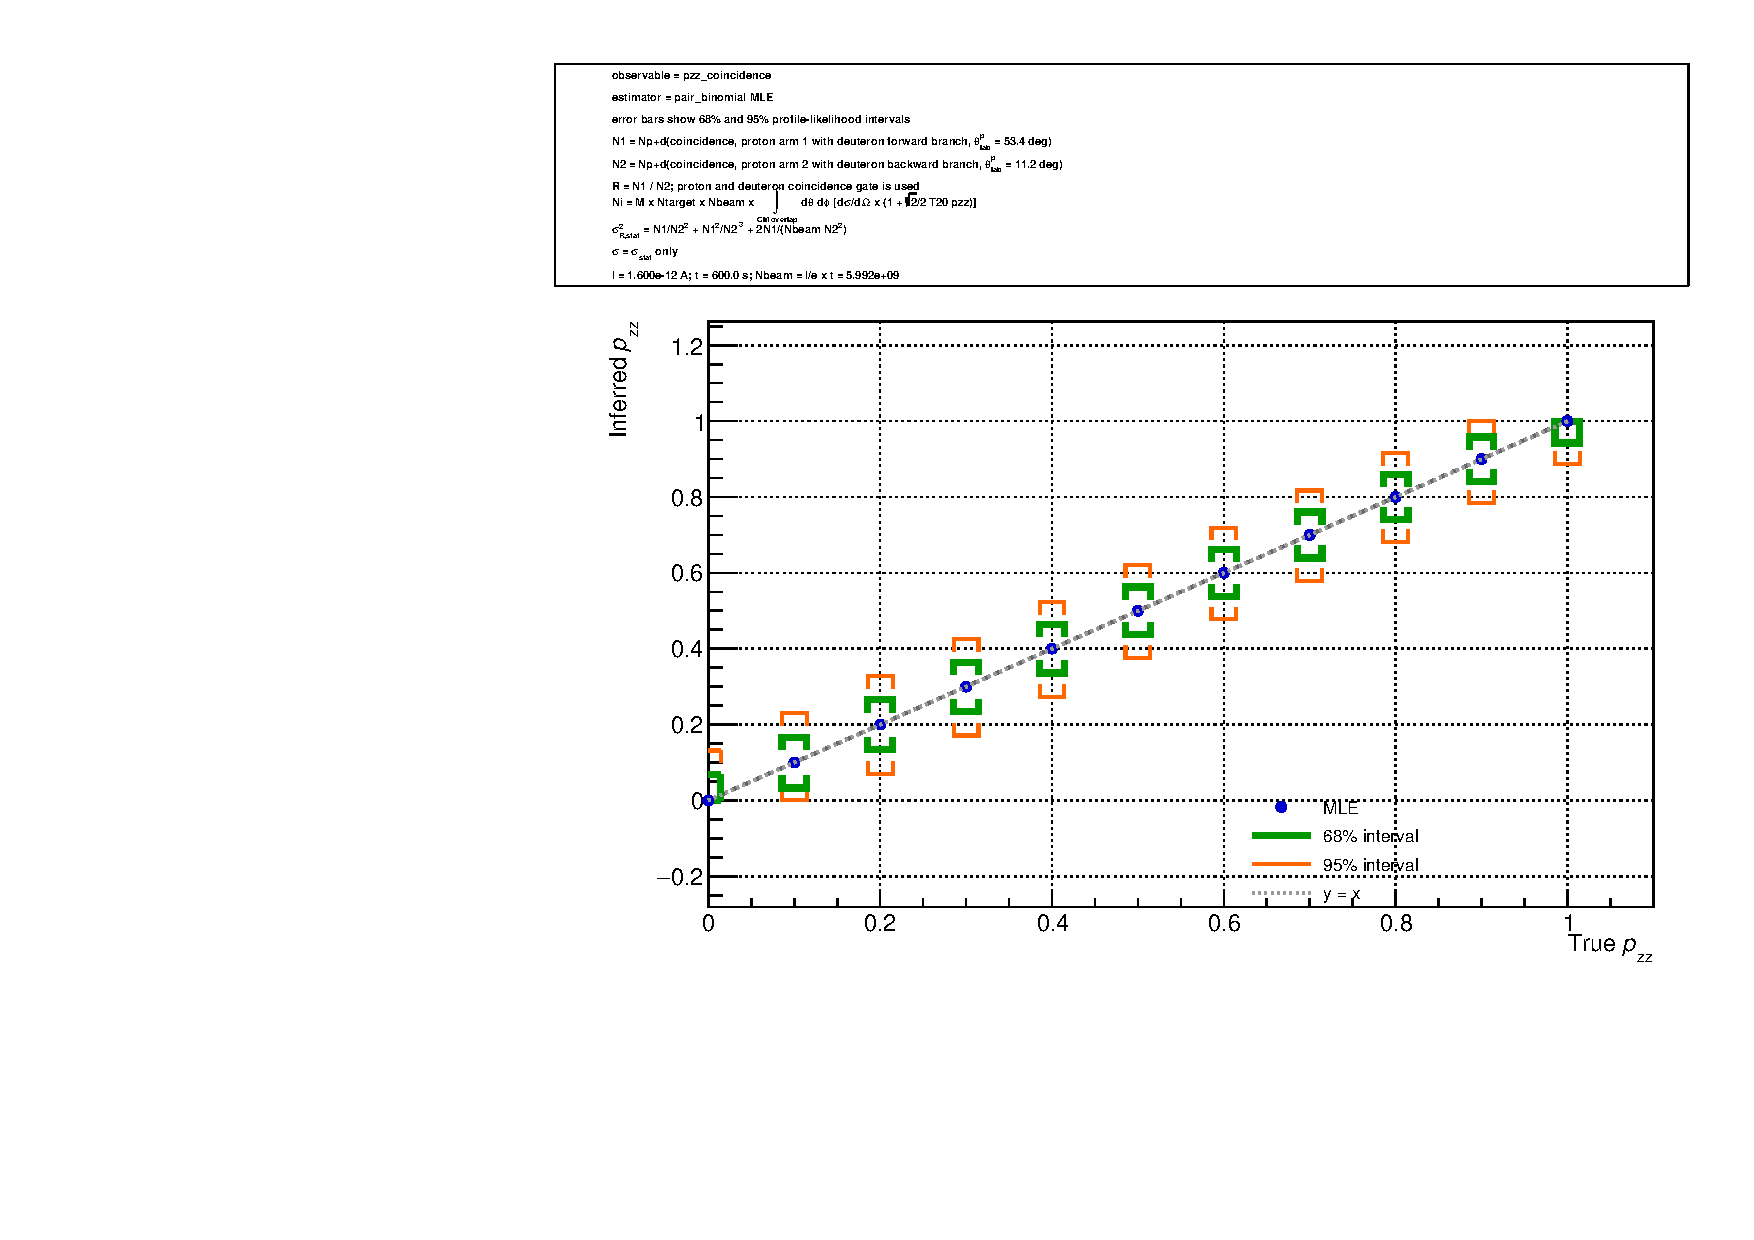
\includegraphics[width=\linewidth]{./generated/default/ratio_coincidence/10min/Inferred_pzz_vs_true_pzz.pdf}
        \caption{\SI{10}{min}.}
    \end{subfigure}
    \begin{subfigure}[t]{0.32\textwidth}
        \centering
        
\includegraphics[width=\linewidth]{./generated/default/ratio_coincidence/1h/Inferred_pzz_vs_true_pzz.pdf}
        \caption{\SI{1}{h}.}
    \end{subfigure}
    \begin{subfigure}[t]{0.32\textwidth}
        \centering
        
\includegraphics[width=\linewidth]{./generated/default/ratio_coincidence/3h/Inferred_pzz_vs_true_pzz.pdf}
        \caption{\SI{3}{h}.}
    \end{subfigure}
    \caption{Beam-time dependence of the MLE reconstruction for the coupled $p+d$ coincidence $p_{zz}$ observable. The horizontal axis (true polarization) is the forward-model input used to generate expected counts/expected ratio, not a fluctuated single-shot measurement.}
    \label{fig:pzz_duration_inference}
\end{figure}

\begin{figure}[htbp]
    \centering
    \begin{subfigure}[t]{0.32\textwidth}
        \centering
        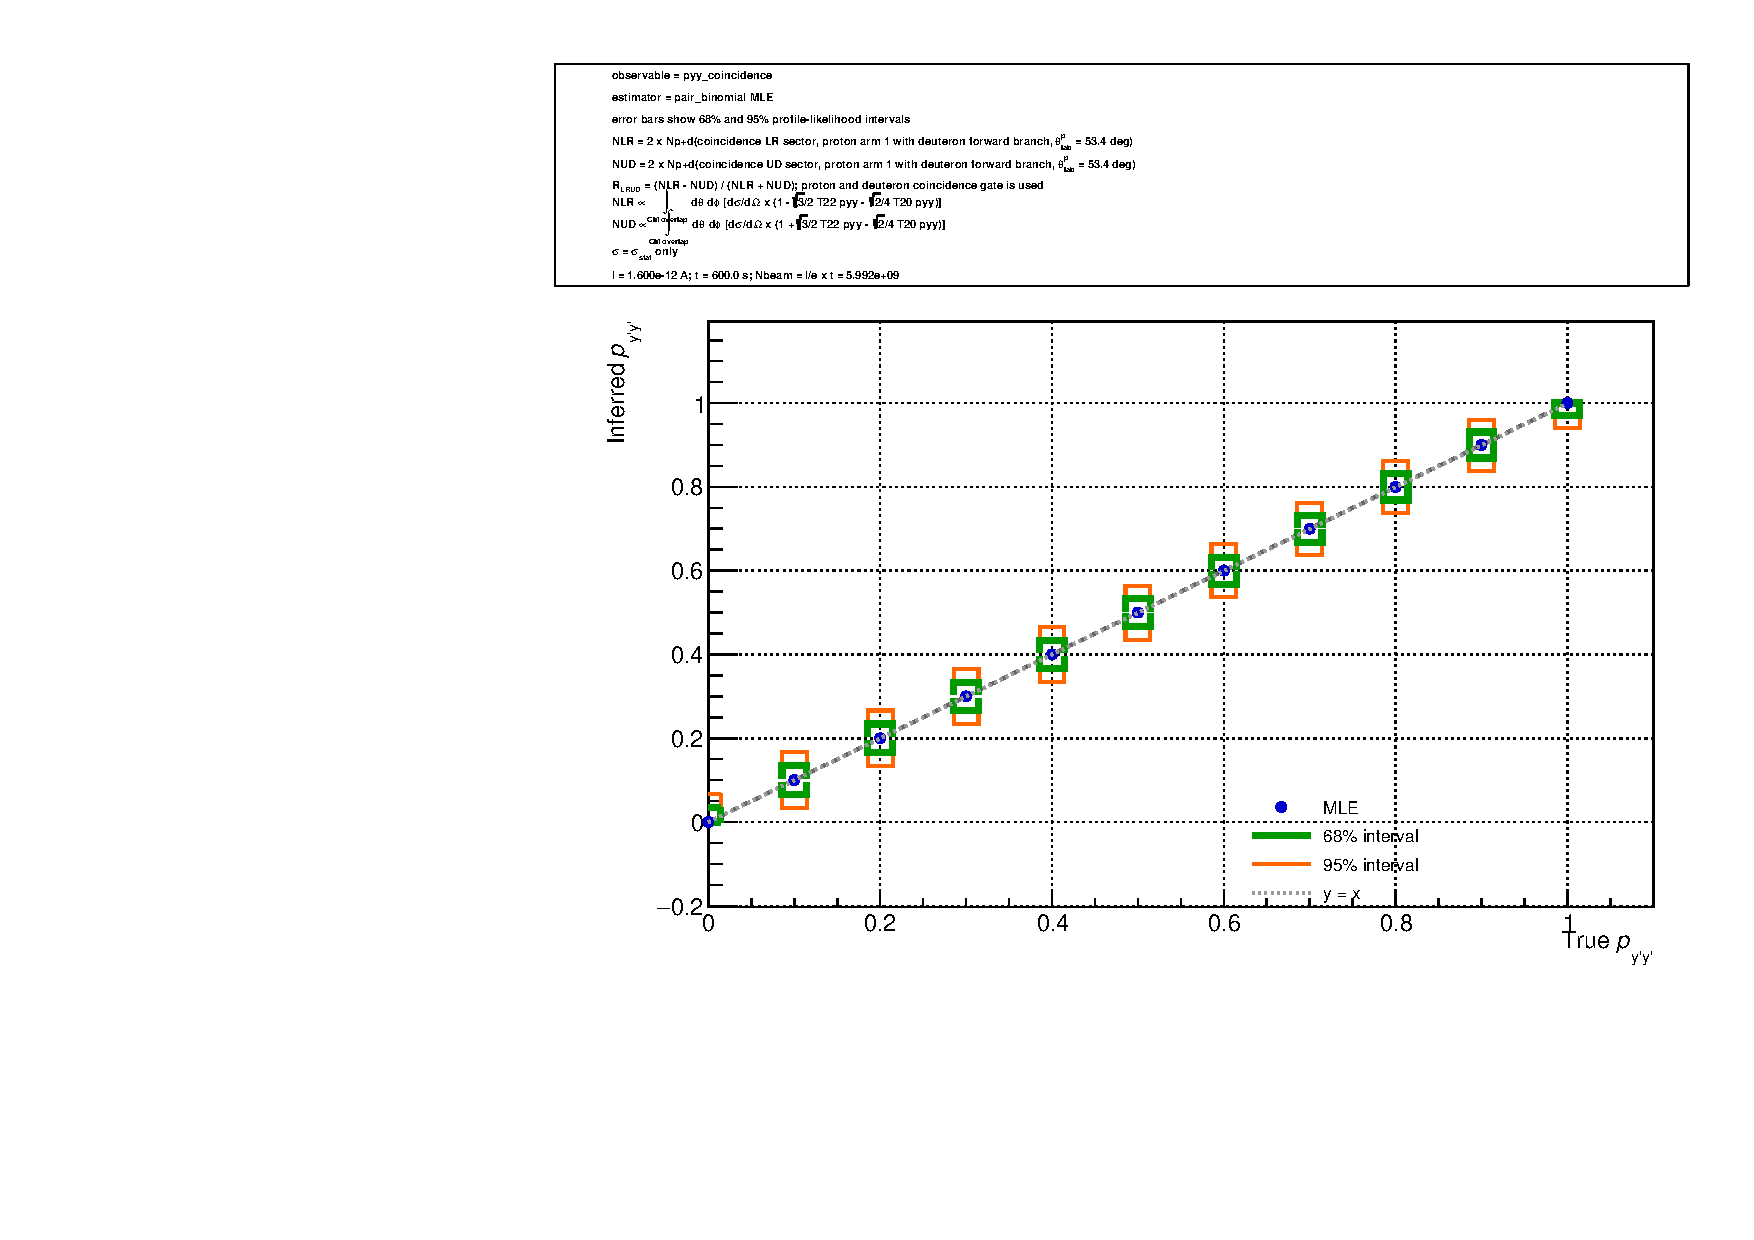
\includegraphics[width=\linewidth]{./generated/default/lrud_coincidence/10min/Inferred_pyy_vs_true_pyy.pdf}
        \caption{\SI{10}{min}.}
    \end{subfigure}
    \begin{subfigure}[t]{0.32\textwidth}
        \centering
        
\includegraphics[width=\linewidth]{./generated/default/lrud_coincidence/1h/Inferred_pyy_vs_true_pyy.pdf}
        \caption{\SI{1}{h}.}
    \end{subfigure}
    \begin{subfigure}[t]{0.32\textwidth}
        \centering
        
\includegraphics[width=\linewidth]{./generated/default/lrud_coincidence/3h/Inferred_pyy_vs_true_pyy.pdf}
        \caption{\SI{3}{h}.}
    \end{subfigure}
    \caption{Beam-time dependence of the MLE reconstruction for the coupled $p+d$ gated LR/UD $p_{y'y'}$ observable. The horizontal axis (true polarization) is the forward-model input used to generate expected counts/expected asymmetry, not a fluctuated single-shot measurement.}
    \label{fig:pyy_duration_inference}
\end{figure}

\begin{figure}[htbp]
    \centering
    \begin{subfigure}[t]{0.32\textwidth}
        \centering
        
\includegraphics[width=\linewidth]{./generated/default/ratio_proton/3h/Inferred_pzz_vs_true_pzz.pdf}
        \caption{Proton single-arm.}
    \end{subfigure}
    \begin{subfigure}[t]{0.32\textwidth}
        \centering
        
\includegraphics[width=\linewidth]{./generated/default/ratio_deuteron/3h/Inferred_pzz_vs_true_pzz.pdf}
        \caption{Deuteron single-arm.}
    \end{subfigure}
    \begin{subfigure}[t]{0.32\textwidth}
        \centering
        
\includegraphics[width=\linewidth]{./generated/default/ratio_coincidence/3h/Inferred_pzz_vs_true_pzz.pdf}
        \caption{Coupled $p+d$ coincidence.}
    \end{subfigure}
    \caption{MLE reconstruction of $p_{zz}$ from the three paired $N_1/N_2$ observables. The marker is the MLE, the inner bar is the 68\% interval, and the outer bar is the 95\% interval. The true-polarization axis corresponds to forward expected observables.}
    \label{fig:pzz_inference_triplet}
\end{figure}

\begin{figure}[htbp]
    \centering
    \begin{subfigure}[t]{0.48\textwidth}
        \centering
        
\includegraphics[width=\linewidth]{./generated/default/lrud_scan/3h/Inferred_pyy_vs_true_pyy.pdf}
        \caption{Proton-only LR/UD.}
    \end{subfigure}
    \begin{subfigure}[t]{0.48\textwidth}
        \centering
        
\includegraphics[width=\linewidth]{./generated/default/lrud_coincidence/3h/Inferred_pyy_vs_true_pyy.pdf}
        \caption{Coupled $p+d$ gated LR/UD.}
    \end{subfigure}
    \caption{MLE reconstruction of $p_{y'y'}$ from the LR/UD asymmetry observables. Under the present default geometry the two curves overlap because the coincidence gate does not further shrink the proton-arm-1 acceptance. The true-polarization axis corresponds to forward expected observables.}
    \label{fig:pyy_inference_pair}
\end{figure}

The single-case profile-likelihood plots below show the local inversion behavior for the coupled coincidence observables at the mid-scan point. Using the \SI{3}{h} generated counts, the coupled $p_{zz}$ case gives $N_1 = 47727.8455$, $N_2 = 93414.7100$, and $\hat{p}_{zz}=0.5000$ with a 68\% interval $[0.4852,\,0.5148]$; the coupled $p_{y'y'}$ case gives $N_{LR}=101626.4230$, $N_{UD}=75425.7794$, and $\hat{p}_{y'y'}=0.5000$ with a 68\% interval $[0.4923,\,0.5077]$.

\begin{figure}[htbp]
    \centering
    \begin{subfigure}[t]{0.48\textwidth}
        \centering
        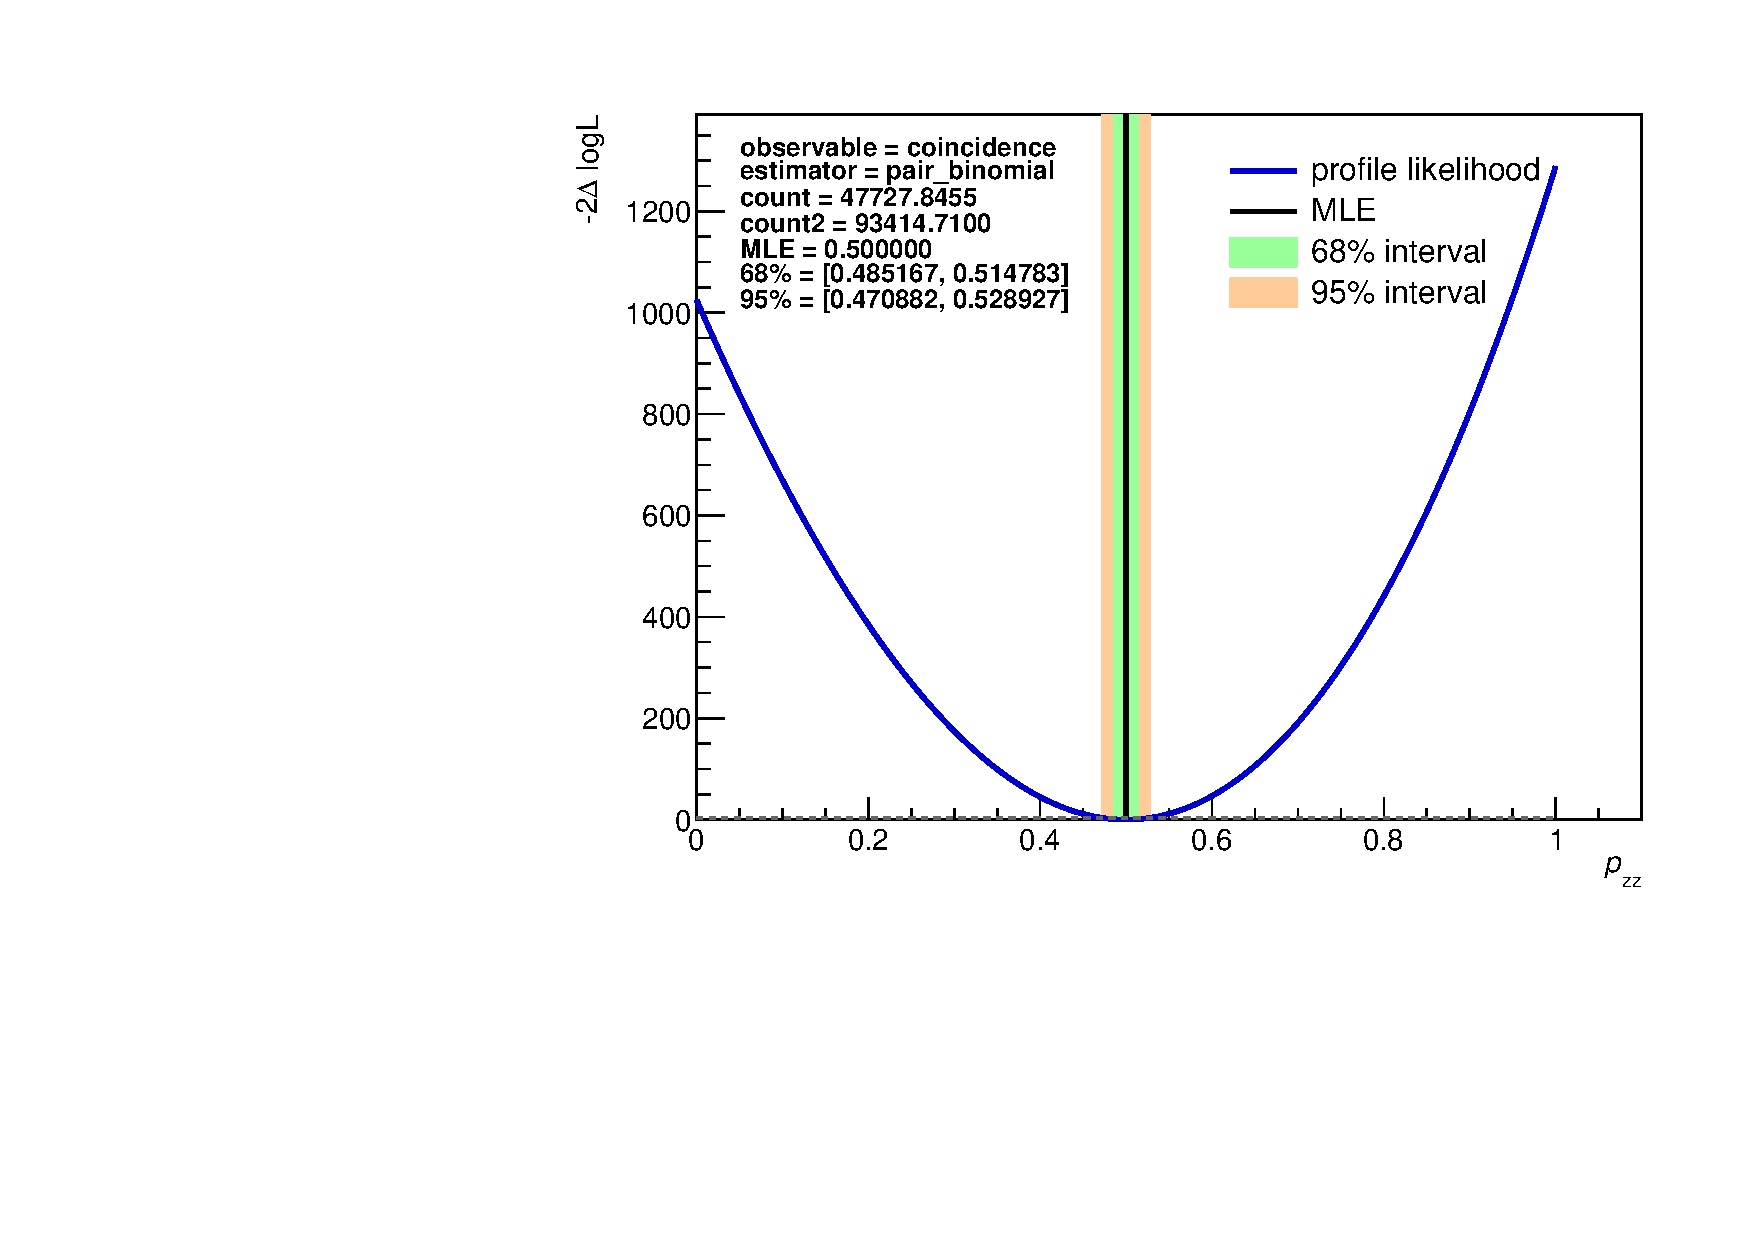
\includegraphics[width=\linewidth]{./generated/default/infer_pzz_plot/coincidence_3h_midscan/Profile_likelihood_vs_pzz.pdf}
        \caption{Profile likelihood for the coupled $p_{zz}$ coincidence ratio.}
    \end{subfigure}
    \begin{subfigure}[t]{0.48\textwidth}
        \centering
        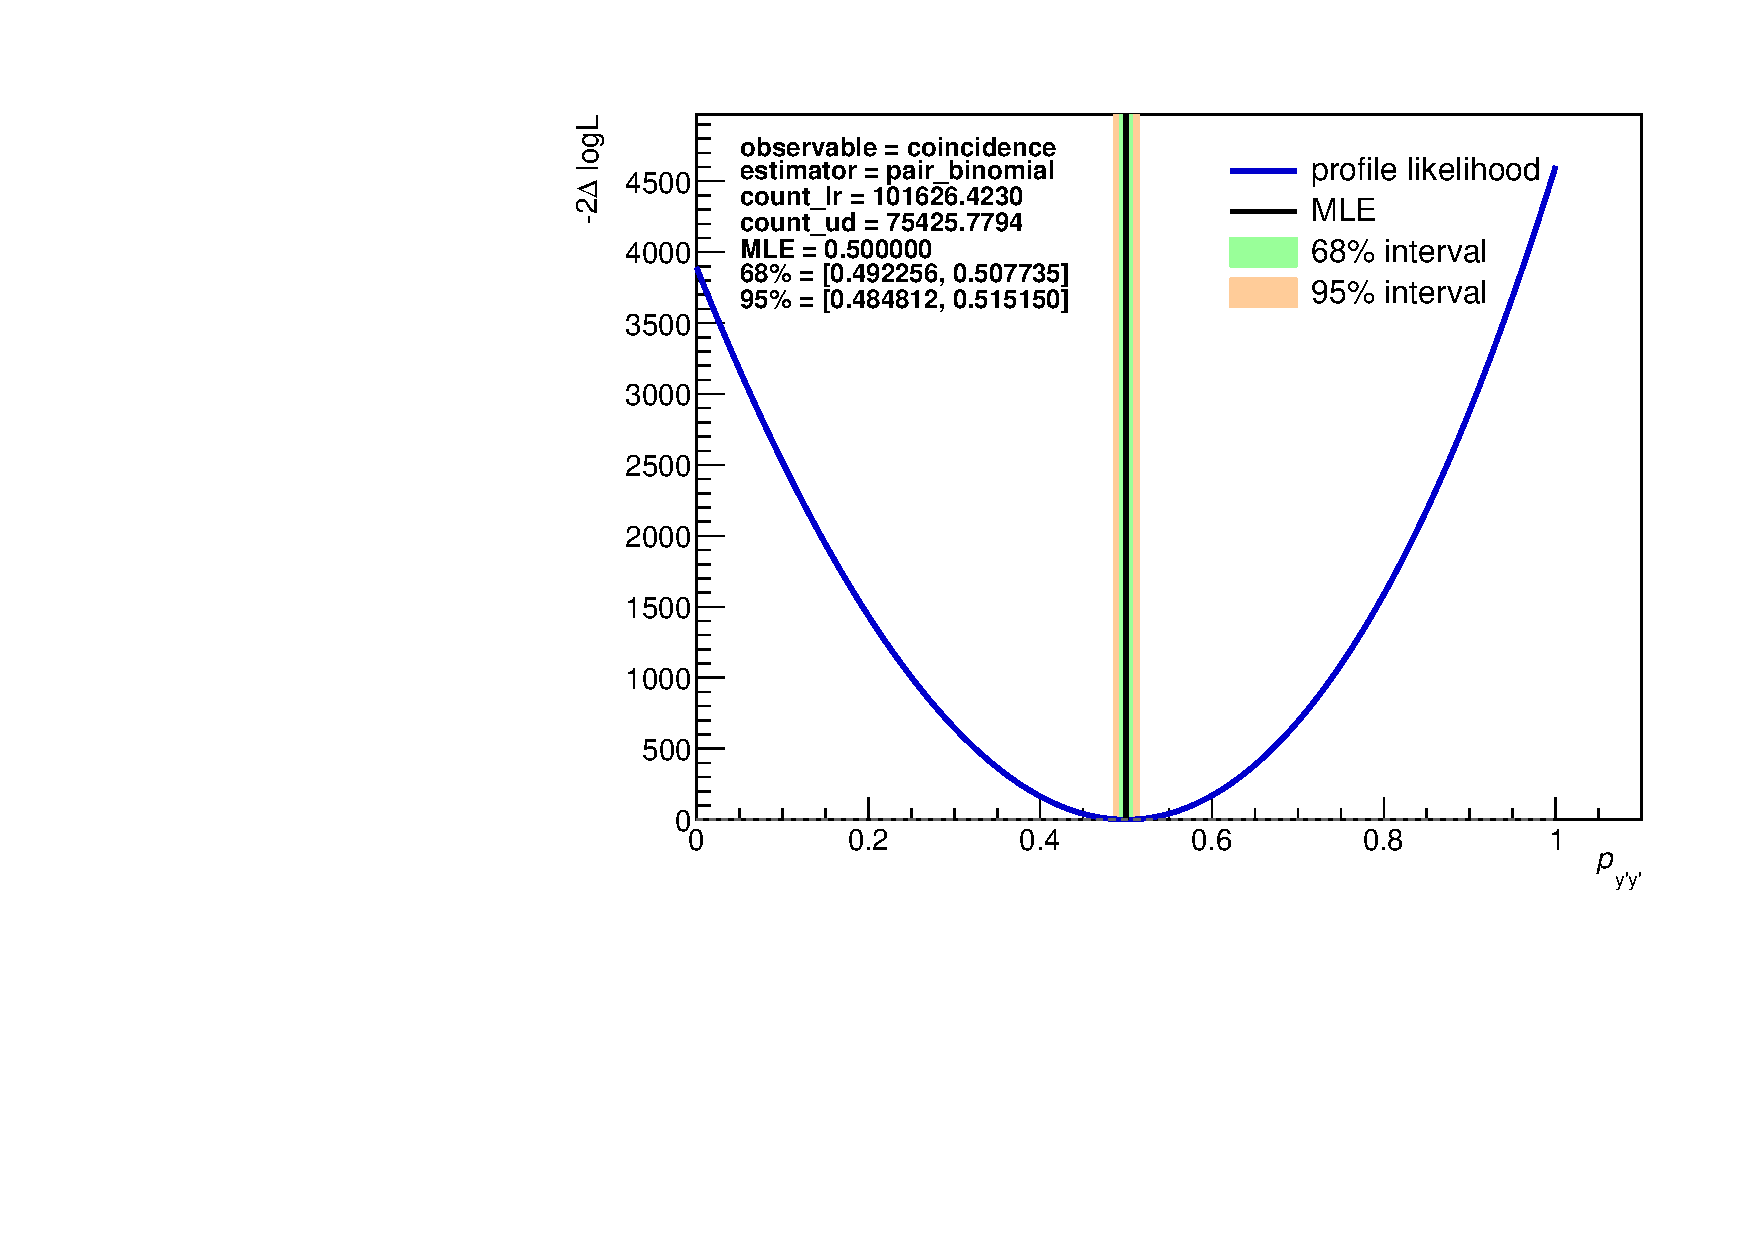
\includegraphics[width=\linewidth]{./generated/default/infer_pyy_plot/coincidence_3h_midscan/Profile_likelihood_vs_pyy.pdf}
        \caption{Profile likelihood for the coupled $p_{y'y'}$ LR/UD asymmetry.}
    \end{subfigure}
    \caption{Example profile-likelihood curves used to invert counts back to polarization. The horizontal likelihood-drop thresholds correspond to the 68\% and 95\% confidence intervals in Equation~\ref{eq:profile_interval}.}
    \label{fig:profile_examples}
\end{figure}

\section{BigRIPS Slits and the Possible F0--F13 Intensity Difference}

The note \texttt{docs/bigreps\_slits/filter\_bigreps.zh.md} explains the essential point: BigRIPS slits remove large-angle particles and momentum-tail particles. Therefore the downstream beam intensity is reduced whenever the transported phase-space distribution exceeds the accepted angular or momentum envelope. Using the usual upstream/downstream shorthand, the transmitted intensity can be written as
\begin{equation}
\label{eq:f0_f13_transport}
    I_{F13} = I_{F0}\,T_{x'}\,T_{y'}\,T_{\delta}\,T_{\mathrm{misc}},
\end{equation}
where $T_{x'}$, $T_{y'}$, and $T_{\delta}$ are the horizontal-angle, vertical-angle, and momentum transmission factors, and $T_{\mathrm{misc}}$ collects residual losses from halo scraping, aperture limitation, optics mismatch, and diagnostics.

If the upstream distributions are approximately Gaussian, a useful first estimate is
\begin{equation}
\label{eq:gaussian_transmission}
    T_{u} \simeq \mathrm{erf}\!\left(\frac{u_{\max}}{\sqrt{2}\sigma_u}\right),
    \qquad
    u \in \{x',\,y',\,\delta\},
\end{equation}
so the F0--F13 intensity difference is controlled directly by how the incoming beam widths compare with the slit settings and beamline acceptance. The internal BigRIPS note summarized in this repository quotes the nominal acceptance scales
\begin{equation}
    |x'| \lesssim \SI{40}{mrad},
    \qquad
    |y'| \lesssim \SI{50}{mrad},
    \qquad
    |\delta| \lesssim 3\%.
\end{equation}

For the present experiment this point needs one extra qualification: we are transporting a primary deuteron beam, not a secondary fragment cocktail. Because of that, the F0--F13 loss budget is qualitatively different from the standard radioactive-beam case.
\begin{enumerate}
    \item There is no production-target yield penalty between F0 and F13. The dominant loss is transport acceptance, not fragment production.
    \item The remaining losses are still real: slit cuts on large-angle particles, momentum-tail cleaning, halo scraping, and mismatch to the separator optics can all reduce the transmitted intensity.
    \item Therefore a moderate F0--F13 difference is entirely plausible even for a primary deuteron beam, but an order-of-magnitude drop would usually imply intentionally tight slits or a poor phase-space match rather than ``ordinary'' transport alone.
    \item In practical terms, if the beam emittance and momentum spread are comfortably smaller than the open BigRIPS acceptance, one expects $I_{F13}$ to remain close to $I_{F0}$. If the slits are narrowed to clean up halo or momentum tails, the transmitted intensity can decrease noticeably while the downstream beam quality improves.
    \item The statements in this section are a transport-based inference from the slit-acceptance model available in the repository, not a direct F0/F13 machine log. A numerical F0/F13 ratio would still require the actual slit settings and the measured upstream $(x',y',\delta)$ distributions of the deuteron beam.
    \end{enumerate}

In short, for this primary deuteron-beam use case the physically relevant question is not ``is there a secondary-beam production loss?'' but ``how much of the incoming deuteron phase space is intentionally or unintentionally clipped before F13?'' That is the mechanism that can generate an observable F0--F13 intensity gap here.



\bibliographystyle{plain}
\bibliography{references} % 如需参考文献，请在同目录添加 references.bib

\end{document}
